\documentclass[10pt]{article}
\usepackage[margin=2cm]{geometry}
\usepackage{amsmath,amssymb}
\usepackage{booktabs,multirow}
\usepackage{graphicx}
\usepackage{xcolor}
\usepackage{caption}
\usepackage[hidelinks]{hyperref}
\captionsetup{font=small,labelfont=bf}
\makeatletter\let\inputrows\@@input\makeatother
\setlength{\parskip}{3pt}\setlength{\parindent}{0pt}

\title{\textbf{CT-KAE on transonic flow: reference and back001}}
\date{30 October 2026}
\author{}

\begin{document}
\maketitle
\vspace{-2.5em}

\section*{Models}
Both are the same continuous-time Koopman autoencoder. A CNN encoder maps two input frames
($\Delta t=0.1$) and the Mach number to $z\in\mathbb R^{256}$. The latent evolves exactly linearly,
$z(\tau)=e^{\tau A(\mathrm{Ma})}z_0$, with $A$ block-diagonal: 128 damped oscillators, decay
$\gamma\ge0$. A FiLM-conditioned CNN decoder maps $z$ back to the four fields. 24.7\,M parameters;
trained 20k steps on the 33 training simulations to reconstruct and to predict 8 frames ahead,
with latent consistency. \textbf{back001} adds backward latent consistency at weight 0.01. Three
seeds each; every number below is a mean over seeds or a 3-seed average, as stated.

\section*{Main results}
\begin{table}[!htbp]
\centering\scriptsize
\caption{Forecasting (MSE $\times10^{-3}$, all frames; LSiM $\times10^{-1}$), data assimilation
(relative $L_2$ of the analysis at $t_0$; df1 headline: 12 problems, 2000 iterations; sweeps: mean
over the points of six sweeps that every method was run on, 31 at $\delta_f=1$ and 37 at
$\delta_f=9$), and inference cost (Tra\_long,
240 steps, batch 1, RTX 4090). Lower is better throughout. Post-processing (MSE-optimal averaging)
and the sharpened mirror average (non-blurring) are described in the next two sections; the effect
of post-processing on DA is in Table~\ref{tab:dapp}. Original KAE: final checkpoint; the published DA numbers used a checkpoint selected on the
DA test set.}
\label{tab:main}
\setlength{\tabcolsep}{3.5pt}
\begin{tabular}{lccccccccccc}
\toprule
 & \multicolumn{3}{c}{MSE} & \multicolumn{3}{c}{LSiM} & \multicolumn{3}{c}{DA error} & ms per\\
\cmidrule(lr){2-4}\cmidrule(lr){5-7}\cmidrule(lr){8-10}
 & ext & int & long & ext & int & long & df1 head. & df1 sweeps & df9 sweeps & step\\
\midrule
\inputrows tab_main.tex
\bottomrule
\end{tabular}
\end{table}

\begin{itemize}\itemsep1pt
\item \textbf{Long rollouts:} at 240 steps both CT-KAEs, without post-processing, have 27--33\% lower
  MSE than ACDM and the U-Nets and 13--18\% lower than the original KAE (46--47\% and 35--36\% with
  it), and stay correlated with the truth over 1000 steps (Fig.~\ref{fig:long}).
\item \textbf{Data assimilation:} both are at least 2$\times$ more accurate than the U-Net and FNO at
  every lead. ACDM\,+\,SDA wins at $\delta_f\le2$. Against the original KAE, back001 is equal at
  short leads and better from $\delta_f=8$; the reference is worse at short leads (Fig.~\ref{fig:da}).
\item \textbf{Short horizon:} without post-processing the U-Nets are best on ext and int. With it the
  reference is best on ext; the U-Nets remain best on int. The sharpened mirror average gives
  almost the same MSE without blurring: on ext the reference has lower MSE than every baseline
  (1.34) and better LSiM than ACDM (1.20 against 1.29); the U-Nets keep the best LSiM.
\item \textbf{back001 vs reference:} back001 is better on DA, int and long, worse on ext.
  Post-processing removes most of the forecasting differences; the DA advantage remains.
\item \textbf{Sharpness:} even without post-processing the CT-KAE is smoother than the baselines
  (worse LSiM, spectra too shallow). Post-processing improves MSE by blurring further
  (Table~\ref{tab:sharp}). The sharpened mirror average does not blur: LSiM improves on ext and int,
  and on long it stays at the single decode's level (Table~\ref{tab:pp3}).
\end{itemize}

\section*{Post-processing}
All steps act at inference on a trained model. Settings were fixed before the test sets were
scored: mixture width and shrinkage on training rollouts, mirror averaging and the choice of steps
on two proxy models trained with Mach 0.53--0.54 and 0.73--0.77 held out.
\begin{itemize}\itemsep1pt
\item \textbf{Mixture readout.} Average of 5 decodes of the same latent flow run at time scales
  $1+\sigma\xi_q$ (Gauss--Hermite, $\sigma\approx0.04$). Hedges the phase drift of the wake.
\item \textbf{Mirror averaging.} The flow is (nearly) symmetric about the centre line: flip the
  input vertically with $v_y\to-v_y$, forecast, flip back, average with the plain forecast.
\item \textbf{Climatology shrinkage.} Per lead and field, pull the forecast towards the
  Mach-interpolated training mean by a factor fitted on training rollouts. Affects long leads only.
\item \textbf{Seed averaging.} Average the forecasts of three independently trained seeds.
\item \textbf{Cost.} The full pipeline is 30 decodes per step: 7.7\,ms per step against 0.27 for a
  single decode, about the cost of a U-Net and 18$\times$ cheaper than ACDM. Peak memory 0.9\,GB.
\item \textbf{Cost in sharpness.} Every step is an average, which MSE rewards and sharpness does
  not: LSiM and the spectral band errors get worse at every scale (Table~\ref{tab:sharp}). Use it
  when the target is MSE, not realistic fields.
\item \textbf{Tested and rejected} on the proxies: test-time refinement of $z_0$ on the input frames
  (always worse), a mixture over neighbouring Mach numbers (no effect), lead-dependent mixture width,
  Wiener filtering by wavenumber (no better than one factor per lead and field).
\end{itemize}

\begin{table}[!htbp]
\centering\scriptsize
\caption{Each post-processing step added in turn: MSE $\times10^{-3}$ (rows 1--4: mean over the 3
seeds; row 5: one 3-seed average), decoder calls per predicted step and wall clock per step.}
\label{tab:pp}
\begin{tabular}{llccccc}
\toprule
 & & ext & int & long & decodes/step & ms/step\\
\midrule
\inputrows tab_pp.tex
\bottomrule
\end{tabular}
\end{table}

\begin{table}[!htbp]
\centering\scriptsize
\caption{What post-processing costs in sharpness. MSE $\times10^{-3}$ on Tra\_long; LSiM
$\times10^{-1}$; relative error of the $|v|$ spectrum on Tra\_long (240 steps) in the low ($k\le4$),
mid (5--12) and high (13--32) bands, and its mid-band slope. Lower is better except the slope, which
should match the ground truth.}
\label{tab:sharp}
\begin{tabular}{lcccccccc}
\toprule
 & MSE & \multicolumn{3}{c}{LSiM} & \multicolumn{4}{c}{spectrum, Tra\_long}\\
\cmidrule(lr){3-5}\cmidrule(lr){6-9}
 & long & ext & int & long & low & mid & high & slope\\
\midrule
\inputrows tab_sharp.tex
\bottomrule
\end{tabular}
\end{table}

\section*{Non-blurring post-processing: sharpened mirror average}
The aim is to lower the error without blurring.
\begin{itemize}\itemsep1pt
\item \textbf{Readout.} Per seed, average the single decode and the mirrored single decode (no
  mixture). Then rescale the anomaly of the average about the Mach-interpolated training mean, per
  frame, field and radial wavenumber, to the mean band power of the two single decodes. The phases of
  the average are kept and the gain is clipped to $[1,5]$; on the proxies the clip never binds within 58 leads. With 3 seeds, all
  6 single decodes are averaged and their mean power is the target. Cost: 6 decodes per step and one
  FFT pair per frame.
\item \textbf{Selection.} Candidates were scored on the proxies' held-out Mach numbers (7
  simulations; 28 windows of 58 leads and 7 of 238): the mirror, mixture and mixture\,+\,mirror
  averages; the latent average of the mixture nodes; re-sharpening of the mirror and mixture\,+\,mirror averages
  (gain exponent 0.5 or 1, clip 2 or 5); Fourier amplitude averaging with the phase of the mean; and
  rank-preserving quantile mapping. The rule was fixed before scoring: LSiM no worse than the single
  decode and band power at most 0.05\,dex lower, on both proxies and both horizons; then lowest MSE.
  Strictly, no candidate passes, because at 238 leads every average raises LSiM. The sharpened mirror
  average is the only one within 1.4\,SE everywhere (reference proxy, long: LSiM $+0.07\pm0.05$). At 58 leads it
  lowers MSE by 9\% and LSiM by 0.10--0.11 on both proxies. The proxies have one seed, so seed
  averaging is not validated there.
\item \textbf{Test} (Table~\ref{tab:pp3}; per seed, paired against the single decode, SE over 3 seeds).
  On ext and int, MSE falls by 10--23\% per seed (15--30\% with the 3-seed average) and LSiM by
  0.10--0.16; the high-band power ratio stays within 0.03\,dex of the single decode. On long, MSE falls
  by 0.19--0.26 (1--2 SE) and LSiM rises by 0.05 (within 1 SE). Over 1000 steps the mean $v_x$ correlation is 0.705 (reference) and 0.699 (back001), against 0.691
  and 0.682 for the single decode and 0.730 and 0.722 for post-processing (Fig.~\ref{fig:long}).
\item \textbf{Against post-processing} (3 seeds, reference): MSE 1.34 / 2.57 / 15.81 against
  1.31 / 2.45 / 11.87 (ext / int / long); LSiM 1.20 / 1.53 / 4.07 against 1.73 / 1.86 / 7.24. Use the
  sharpened mirror average when realistic fields matter. The long-horizon MSE gain of post-processing
  comes only from blurring.
\item \textbf{Rejected.} The latent average of the mixture nodes equals the single decode at 58 leads
  and blurs at 238. Sharpening the
  mixture\,+\,mirror average keeps the mixture's loss at long leads. Fourier amplitude averaging is
  close to sharpening but slightly worse. Quantile mapping fixes amplitudes, not scales, so the high band
  still loses power. In an earlier test-set screen, $x$-shift-aligned averaging and the medoid member gained
  nothing. Refinement with the trained ACDM (SDEdit) was not run: each frame would need part of
  ACDM's sampler (142\,ms per step in full), up to $\sim$500$\times$ a single decode.
\end{itemize}

\begin{table}[!htbp]
\centering\scriptsize
\caption{Sharpened mirror average, each step added in turn. MSE $\times10^{-3}$, LSiM $\times10^{-1}$,
and the mean $\log_{10}$ power ratio (prediction / truth) of the $|v|$ spectrum in the high band
(13--32; 0 is exact, negative is smoother). Rows 1--3: mean over 3 seeds; row 4: one 3-seed average;
row 5: paired change of row 3 against row 1, $\pm$ SE over seeds.}
\label{tab:pp3}
\setlength{\tabcolsep}{3pt}
\resizebox{\linewidth}{!}{%
\begin{tabular}{llccccccccccc}
\toprule
 & & \multicolumn{3}{c}{MSE} & \multicolumn{3}{c}{LSiM} & \multicolumn{3}{c}{high-band log ratio} & decodes & ms\\
\cmidrule(lr){3-5}\cmidrule(lr){6-8}\cmidrule(lr){9-11}
 & & ext & int & long & ext & int & long & ext & int & long & /step & /step\\
\midrule
\inputrows tab_pp3.tex
\bottomrule
\end{tabular}}
\end{table}

\textbf{In data assimilation} only mirror averaging applies: 4D-Var is run once in the plain frame and
once in the mirrored frame, and the two analyses are averaged. It cuts the analysis error by 10--16\% for both models at twice the cost
(Table~\ref{tab:dapp}).

\begin{figure}[!htbp]
\centering
\begin{minipage}[b]{0.56\linewidth}\centering
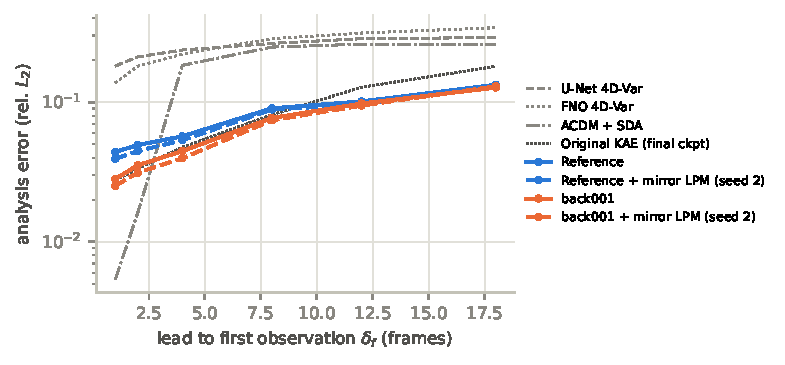
\includegraphics[width=\linewidth]{fig_da.pdf}
\captionof{figure}{Analysis error against the lead $\delta_f$ to the first observation, transonic
flow, $\delta_l=25$, 5 observations, 500 iterations, 8 problems per point.}
\label{fig:da}
\end{minipage}\hfill
\begin{minipage}[b]{0.41\linewidth}\centering\scriptsize
\captionof{table}{Mirror averaging in 4D-Var: analysis error, seed 2 of each model, same problems
as Table~\ref{tab:main}.}
\label{tab:dapp}
\setlength{\tabcolsep}{3pt}
\begin{tabular}{llccc}
\toprule
 & & df1 & df1 & df9\\
 & & head. & sweeps & sweeps\\
\midrule
\inputrows tab_da_pp.tex
\bottomrule
\end{tabular}
\end{minipage}
\end{figure}

\section*{The paper's transonic experiments, re-run}

\begin{table}[!htbp]
\centering\scriptsize
\caption{MSE ($\times10^{-3}$, all fields) at $t=15,30,45,60$ of the 60-step rollouts. CT-KAE
rows without post-processing: mean over 3 seeds. Best per column in bold.}
\label{tab:lead}
\begin{tabular}{lcccccccc}
\toprule
 & \multicolumn{4}{c}{Tra\_ext} & \multicolumn{4}{c}{Tra\_int}\\
\cmidrule(lr){2-5}\cmidrule(lr){6-9}
$t$ & 15 & 30 & 45 & 60 & 15 & 30 & 45 & 60\\
\midrule
\inputrows tab_lead.tex
\bottomrule
\end{tabular}
\end{table}

\begin{figure}[!htbp]
\centering
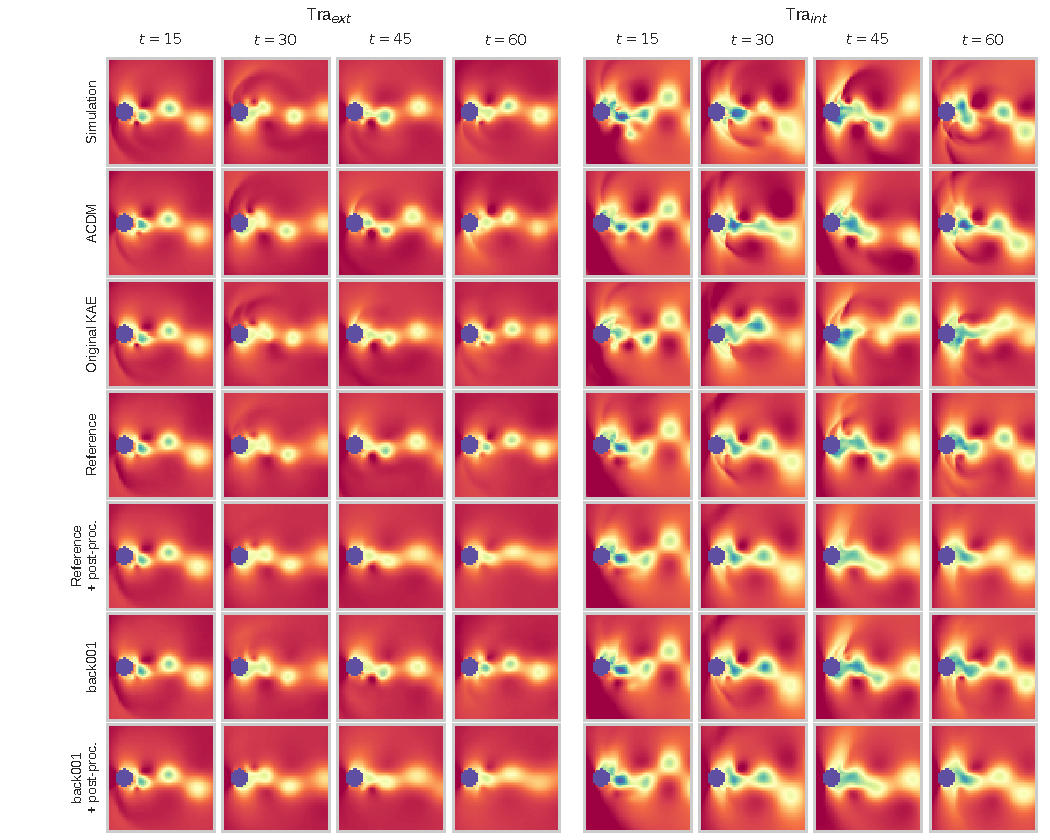
\includegraphics[width=0.85\linewidth]{fig_short.pdf}
\caption{Pressure at $t=15,30,45,60$, first sequence of each test set (paper layout). CT-KAE rows
without post-processing: seed 0; post-processing and sharpened mirror: 3-seed average. Number in each panel: pressure MSE ($\times10^{-3}$) of that
frame over the whole domain; bold is the best model in the column.}
\label{fig:short}
\end{figure}

\textbf{Short horizon.} The U-Nets are best up to $t=30$. On ext the post-processed reference is best
from $t=45$. On int the U-Net$_{ut}$ stays best; at $t=60$ the post-processed CT-KAEs are second
(5.6--5.7 against 4.9), ahead of ACDM (8.5) and the original KAE (15.8).

\begin{figure}[!htbp]
\centering
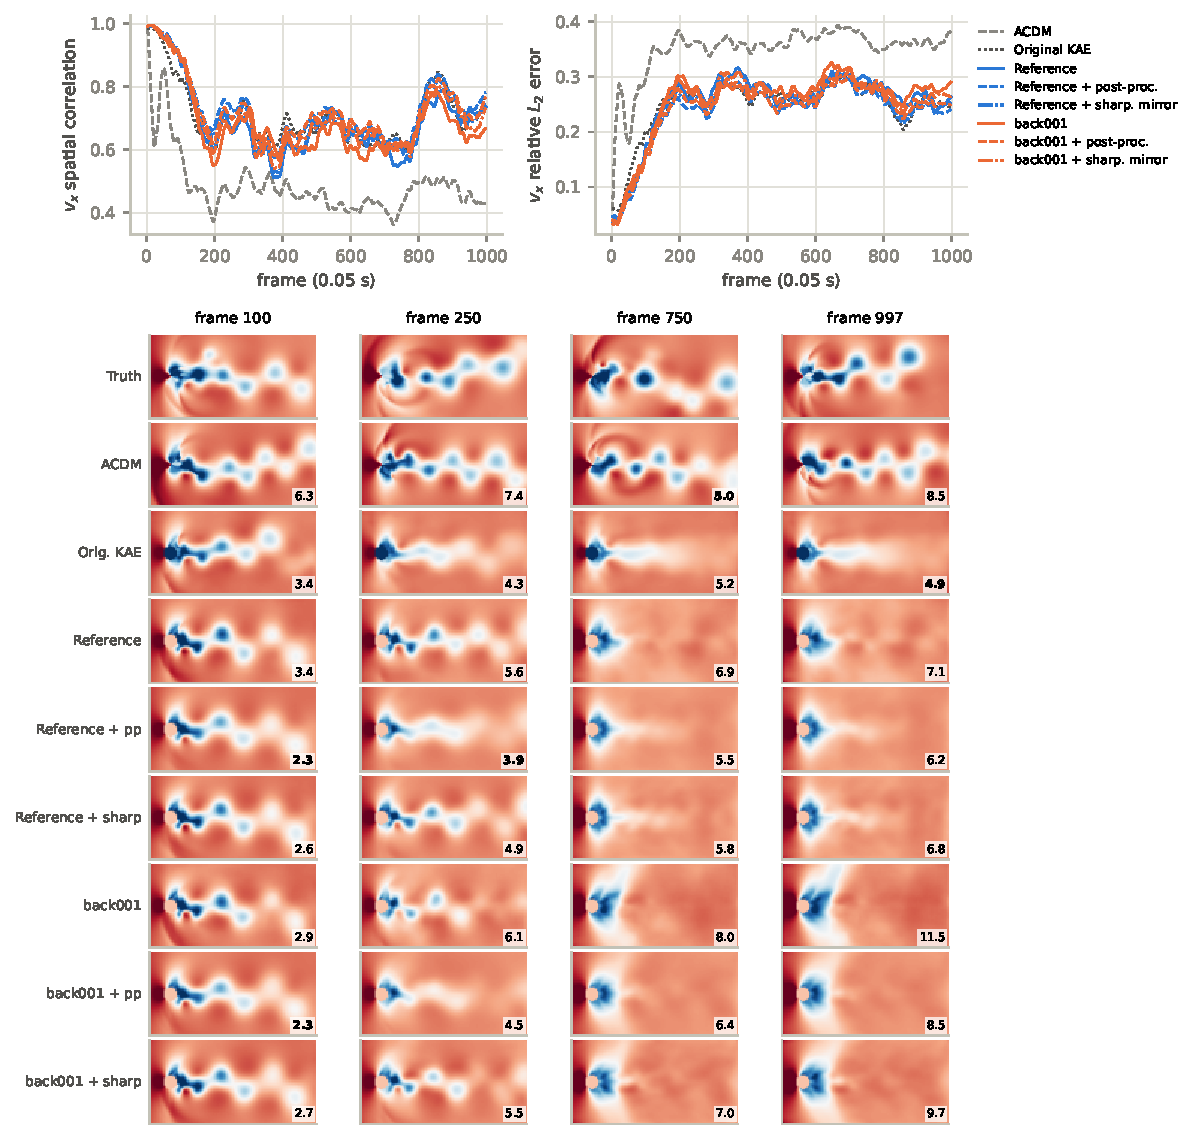
\includegraphics[width=\linewidth]{fig_long.pdf}
\caption{1000-step rollout (Tra\_long simulations, 0.05\,s per frame, 2 trajectories). Top: $v_x$
spatial correlation and relative $L_2$ error per frame. Bottom: pressure, first trajectory.
Post-processing here is the 3-seed average of mixture + mirror, without shrinkage; ``sharp'' is the
3-seed sharpened mirror average. Number in each panel: pressure MSE ($\times10^{-3}$) of that frame; bold is the best in the column.}
\label{fig:long}
\end{figure}

\begin{table}[!htbp]
\centering\scriptsize
\begin{minipage}[t]{0.55\linewidth}\centering
\caption{The latent ODE $\dot y=Ay$ integrated numerically instead of $e^{\tau A}$ (seed 0, single
decode). MSE $\times10^{-3}$.}
\label{tab:solvers}
\begin{tabular}{llccc}
\toprule
 & integrator & ext & int & long\\
\midrule
\inputrows tab_solvers.tex
\bottomrule
\end{tabular}
\end{minipage}\hfill
\begin{minipage}[t]{0.42\linewidth}\centering
\caption{Unseen time step: MSE at leads on the training grid (0.1\,s) and at the half-steps
between them (0.05\,s, never trained on). Mean over 3 seeds.}
\label{tab:dt}
\begin{tabular}{lcccc}
\toprule
 & \multicolumn{2}{c}{ext} & \multicolumn{2}{c}{int}\\
 & 0.1 & 0.05 & 0.1 & 0.05\\
\midrule
\inputrows tab_dt.tex
\bottomrule
\end{tabular}
\end{minipage}
\end{table}

\begin{table}[!htbp]
\centering\scriptsize
\caption{Spectrum of $|v|$: relative error in the low ($k\le4$), mid (5--12) and high (13--32)
wavenumber bands and the fitted mid-band slope.}
\label{tab:spec}
\begin{tabular}{lcccccccc}
\toprule
 & \multicolumn{4}{c}{Tra\_int (60 steps)} & \multicolumn{4}{c}{Tra\_long (240 steps)}\\
\cmidrule(lr){2-5}\cmidrule(lr){6-9}
 & low & mid & high & slope & low & mid & high & slope\\
\midrule
\inputrows tab_spectral.tex
\bottomrule
\end{tabular}
\end{table}

\begin{figure}[!htbp]
\centering
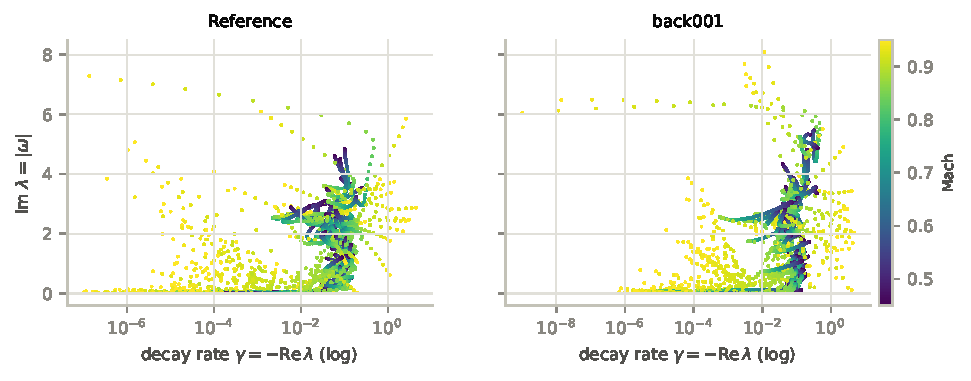
\includegraphics[width=0.9\linewidth]{fig_eigen.pdf}
\caption{Generator eigenvalues $\lambda=-\gamma\pm i\omega$ for Mach 0.45--0.95 (seed 0).}
\label{fig:eigen}
\end{figure}

\textbf{Findings.}
\begin{itemize}\itemsep1pt
\item \textbf{Integrators.} RK4 matches the exact exponential up to $\Delta t=0.3$; explicit Euler
  diverges on long rollouts (from $\Delta t=0.05$ for back001), as the oscillators are almost undamped.
\item \textbf{Unseen time step.} Forecasts between the training time steps are as accurate as on
  them (Table~\ref{tab:dt}).
\item \textbf{Spectra.} The CT-KAE spectra are too shallow and its band errors are 3--7$\times$
  those of ACDM and the U-Net (but well below FNO's on long rollouts); post-processing worsens them. The CT-KAE's MSE advantage on long
  rollouts comes from tracking phase, not from resolving small scales.
\item \textbf{Not re-run:} the original KAE's loss and LoRA ablations need retraining; the CT-KAE's
  own ablation study (in the full report) replaces them.
\end{itemize}

\end{document}
